\documentclass{article}
%\usepackage{ctex}
\usepackage{amsmath}
\usepackage{amsfonts}

\usepackage{graphicx}                                                           
\usepackage{float}

\usepackage{listings}
\usepackage{xcolor}

\usepackage{algorithm}
%\usepackage{algorithmic}
\usepackage{algorithmicx} 
\usepackage{algpseudocode}

\definecolor{mygreen}{rgb}{0,0.6,0}
\definecolor{mygray}{rgb}{0.5,0.5,0.5}
\definecolor{mymauve}{rgb}{0.58,0,0.82}
\lstset{
 backgroundcolor=\color{lightgray}, 
 basicstyle = \footnotesize,       
 breakatwhitespace = false,        
 breaklines = true,                 
 captionpos = b,                    
 commentstyle = \color{mygreen}\bfseries,
 extendedchars = false,             
 frame =shadowbox, 
 framerule=0.5pt,
 keepspaces=true,
 keywordstyle=\color{blue}\bfseries, % keyword style
 language = C++,                     % the language of code
 otherkeywords={string}, 
 numbers=left, 
 numbersep=5pt,
 numberstyle=\tiny\color{mygray},
 rulecolor=\color{black},         
 showspaces=false,  
 showstringspaces=false, 
 showtabs=false,    
 stepnumber=1,         
 stringstyle=\color{mymauve},        % string literal style
 tabsize=2,          
 title=\lstname                      
}


\title{\textbf{Chapter2 Programming}}
\author{Zhehao Chen 3220103172
  \thanks{Electronic address: \texttt{3220103172@zju.edu.cn}}}
\date{\today}

\begin{document}

\maketitle

\section{Implementation Analysis of Base Class: Interpolation}

\subsection{Design Implementation}
The abstract base class \texttt{Interpolation} defines a generic framework for interpolation methods. This is achieved through a common interface, which includes two pure virtual functions that must be implemented by all derived classes. The class also manages shared data members for storing input values.

\begin{itemize}
    \item \textbf{Data Member Implementation:}
    \begin{itemize}
        \item \texttt{x\_values}: A protected vector holding the x-coordinates of the data points, accessible by derived classes for interpolation calculations.
        \item \texttt{y\_values}: A protected vector storing the corresponding y-values, ensuring encapsulation of the input data while still accessible to derived classes.
        \item The constructor validates that the sizes of \texttt{x\_values} and \texttt{y\_values} match, ensuring consistency and preventing runtime errors.
    \end{itemize}
    
    \item \textbf{Virtual Function Specifications:}
    \begin{itemize}
        \item \texttt{interpolate()}: A pure virtual function that must return the interpolated value for a given input x. The derived classes will implement this according to their respective interpolation algorithms.
        \item \texttt{getExpression()}: Another pure virtual function that returns the symbolic representation of the interpolation polynomial as a string.
        \item A virtual destructor ensures that any dynamic memory allocated in derived classes is properly released during object destruction.
    \end{itemize}
\end{itemize}

\section{Detailed Implementation of Newton Interpolation}

\subsection{Interpolate Function Implementation}
The Newton Interpolation method relies on divided differences to construct the interpolation polynomial.

\begin{itemize}
    \item \textbf{Divided Differences Computation:}
    Divided differences are recursively computed using the formula:
    \[
    f[x_i,\ldots,x_{i+k}] = \frac{f[x_{i+1},\ldots,x_{i+k}] - f[x_i,\ldots,x_{i+k-1}]}{x_{i+k} - x_i}
    \]
    
    \item \textbf{Implementation Strategy:}
    \begin{enumerate}
        \item \textbf{Table Initialization:} A vector \texttt{dd} is initialized, where \texttt{dd[i]} holds the divided differences for each degree. Initially, \texttt{dd[i]} is set to \texttt{y\_values[i]}.
        
        \item \textbf{Coefficient Calculation:} The divided differences are calculated iteratively. For each order \( j \), the vector is updated in place, reducing the space complexity by avoiding the need for a full table. The new value of \texttt{dd[i]} is computed using the formula for divided differences.
        
        \item \textbf{Polynomial Evaluation:} The final interpolation polynomial is evaluated by starting with the first divided difference, then progressively multiplying by \( (x - x_k) \) terms and accumulating the result.
    \end{enumerate}
\end{itemize}

\subsection{GetExpression Function Implementation}
The function generates the symbolic expression for the Newton interpolation polynomial.

\begin{itemize}
    \item \textbf{Expression Building Process:}
    \begin{enumerate}
        \item \textbf{Coefficient Generation:} The divided differences table is recomputed, and the coefficients are stored in a temporary vector. To improve readability, coefficients smaller than a threshold (e.g., \(1e^{-10}\)) are ignored.
        
        \item \textbf{String Construction:} The expression is constructed using a \texttt{stringstream}. For each coefficient, its sign is handled separately to ensure proper formatting. The terms \( (x - x_i) \) are progressively appended to build the final expression.
    \end{enumerate}
\end{itemize}

\section{Detailed Implementation of Chebyshev Interpolation}

\subsection{Node Generation Implementation}
Chebyshev interpolation uses nodes based on the roots of Chebyshev polynomials to minimize the interpolation error.

\begin{itemize}
    \item \textbf{Chebyshev Nodes Calculation:}
    The nodes are calculated as:
    \[
    x_i = \frac{a + b}{2} + \frac{b - a}{2} \cos\left(\frac{2i + 1}{2n} \pi\right)
    \]
    where \(a\) and \(b\) are the interpolation interval endpoints, and \(n\) is the number of nodes.
    
    \item \textbf{Implementation Strategy:}
    The calculated nodes are mapped from the interval \([-1, 1]\) to \([a, b]\) using a linear transformation. These nodes are stored in ascending order to facilitate efficient interpolation.
\end{itemize}

\section{Detailed Implementation of Bezier Interpolation}

\subsection{Point Structure Implementation}
In Bezier interpolation, the \texttt{Point} class encapsulates control points for the curve and provides operator overloading to simplify vector arithmetic operations.

\begin{itemize}
    \item \textbf{Operator Overloading:}
    The \texttt{Point} class overloads arithmetic operators for vector addition and scalar multiplication, crucial for manipulating control points in the Bezier algorithm.
    \begin{enumerate}
        \item \textbf{Addition (\texttt{+}):} Adds two \texttt{Point} objects by adding their corresponding x and y coordinates. This operator is frequently used in the iterative process of calculating intermediate points along the curve.
        
        \item \textbf{Scalar Operations:} Supports both multiplication and division by a scalar. These operations are critical for scaling control points when computing the convex combinations in De Casteljau’s algorithm.
    \end{enumerate}
\end{itemize}

\subsection{Curve Fitting Implementation}
Bezier curve fitting involves generating control points and then using them to define the segments of the curve.

\begin{itemize}
    \item \textbf{Control Point Generation:}
    The control points are calculated by manipulating the tangents of the input data points. For each segment, a set of four control points \( q_0, q_1, q_2, q_3 \) is determined.
    \begin{enumerate}
        \item \textbf{Tangent Processing:} The tangent vectors are scaled by \(1/3\) to ensure smooth transitions between segments while maintaining \(C^1\) continuity. The control points are calculated based on these scaled tangents.
        
        \item \textbf{Curve Segment Construction:} Each segment of the Bezier curve is represented as a cubic Bezier defined by its four control points. The segments are connected smoothly by sharing endpoints between adjacent segments.
    \end{enumerate}
\end{itemize}

\subsection{Curve Evaluation Implementation}
The Bezier curve is evaluated using De Casteljau's algorithm, which recursively computes intermediate points based on the parameter \(t\).

\begin{itemize}
    \item \textbf{De Casteljau's Algorithm:}
    \begin{enumerate}
        \item \textbf{Parameter Processing:} The input parameter \(t\) is validated to ensure it lies in the range \([0, 1]\). Powers of \(t\) and \(1 - t\) are computed to simplify the recursive calculation of intermediate points.
        
        \item \textbf{Point Computation:} The algorithm computes weighted averages of control points at each recursion level. By repeatedly interpolating between control points, the algorithm produces the interpolated point on the curve corresponding to the parameter \(t\).
    \end{enumerate}
\end{itemize}


\section{Problem B}

We are tasked with interpolating the Runge function using evenly spaced nodes $x_i = -5 + 10 \frac{i}{n}$, where $n$ is the number of intervals. The values of $n$ used in this experiment are $2, 4, 6, 8$, producing polynomials of different degrees. The aim is to reproduce a graph that illustrates the Runge phenomenon, where the error near the interval edges increases drastically for higher-degree polynomials.

The interpolation function is generated using Newton's method, and the output expression for each polynomial is printed.

\subsection{Code Implementation}

\subsubsection{Function Definitions}

The implementation consists of several key components:

\begin{itemize}
    \item \texttt{generateXValues(int n)}: Generates the x-values for the interpolation nodes. The formula used is $x_i = -5 + 10 \frac{i}{n}$, ensuring evenly spaced nodes across the interval.
    \item \texttt{rungeFunction(double x)}: Defines the Runge function $f(x) = \frac{1}{1+x^2}$.
    \item \texttt{generateYValues(const std::vector<double>\& x\_values)}: Takes the x-values and computes the corresponding y-values using the Runge function.
\end{itemize}

\subsubsection{Newton Interpolation Class}

Newton interpolation is implemented in the class \texttt{NewtonInterpolation}, which is responsible for generating the interpolating polynomial based on divided differences. The method \texttt{getExpression()} returns a string representation of the interpolated polynomial, which is printed for each $n$ value.

The overall structure of the program is designed to loop through the different $n$ values, generate the corresponding interpolation nodes, compute the polynomial, and then display the results.

\subsection{Runge Phenomenon Analysis}

The Runge phenomenon is a well-known issue in polynomial interpolation, particularly when using high-degree polynomials with evenly spaced nodes. As shown in the code and visualized in the resulting plot (Figure~\ref{fig:runge}), the approximation tends to oscillate more drastically near the edges of the interval as $n$ increases. 

The experiment used $n = 2, 4, 6, 8$ to observe this phenomenon. For lower values of $n$, such as $n=2$, the interpolation polynomial closely follows the Runge function, albeit with some deviation at the edges. As $n$ increases, particularly for $n=8$, the oscillations near the boundaries become more severe, a hallmark of the Runge phenomenon.

\subsubsection{Results}

Figure~\ref{fig:runge_plot} shows the output graph of the Runge function and the interpolating polynomials. As the degree of the polynomial increases, the accuracy improves near the center of the interval but worsens significantly near the endpoints.

\begin{figure}[H]
    \centering
    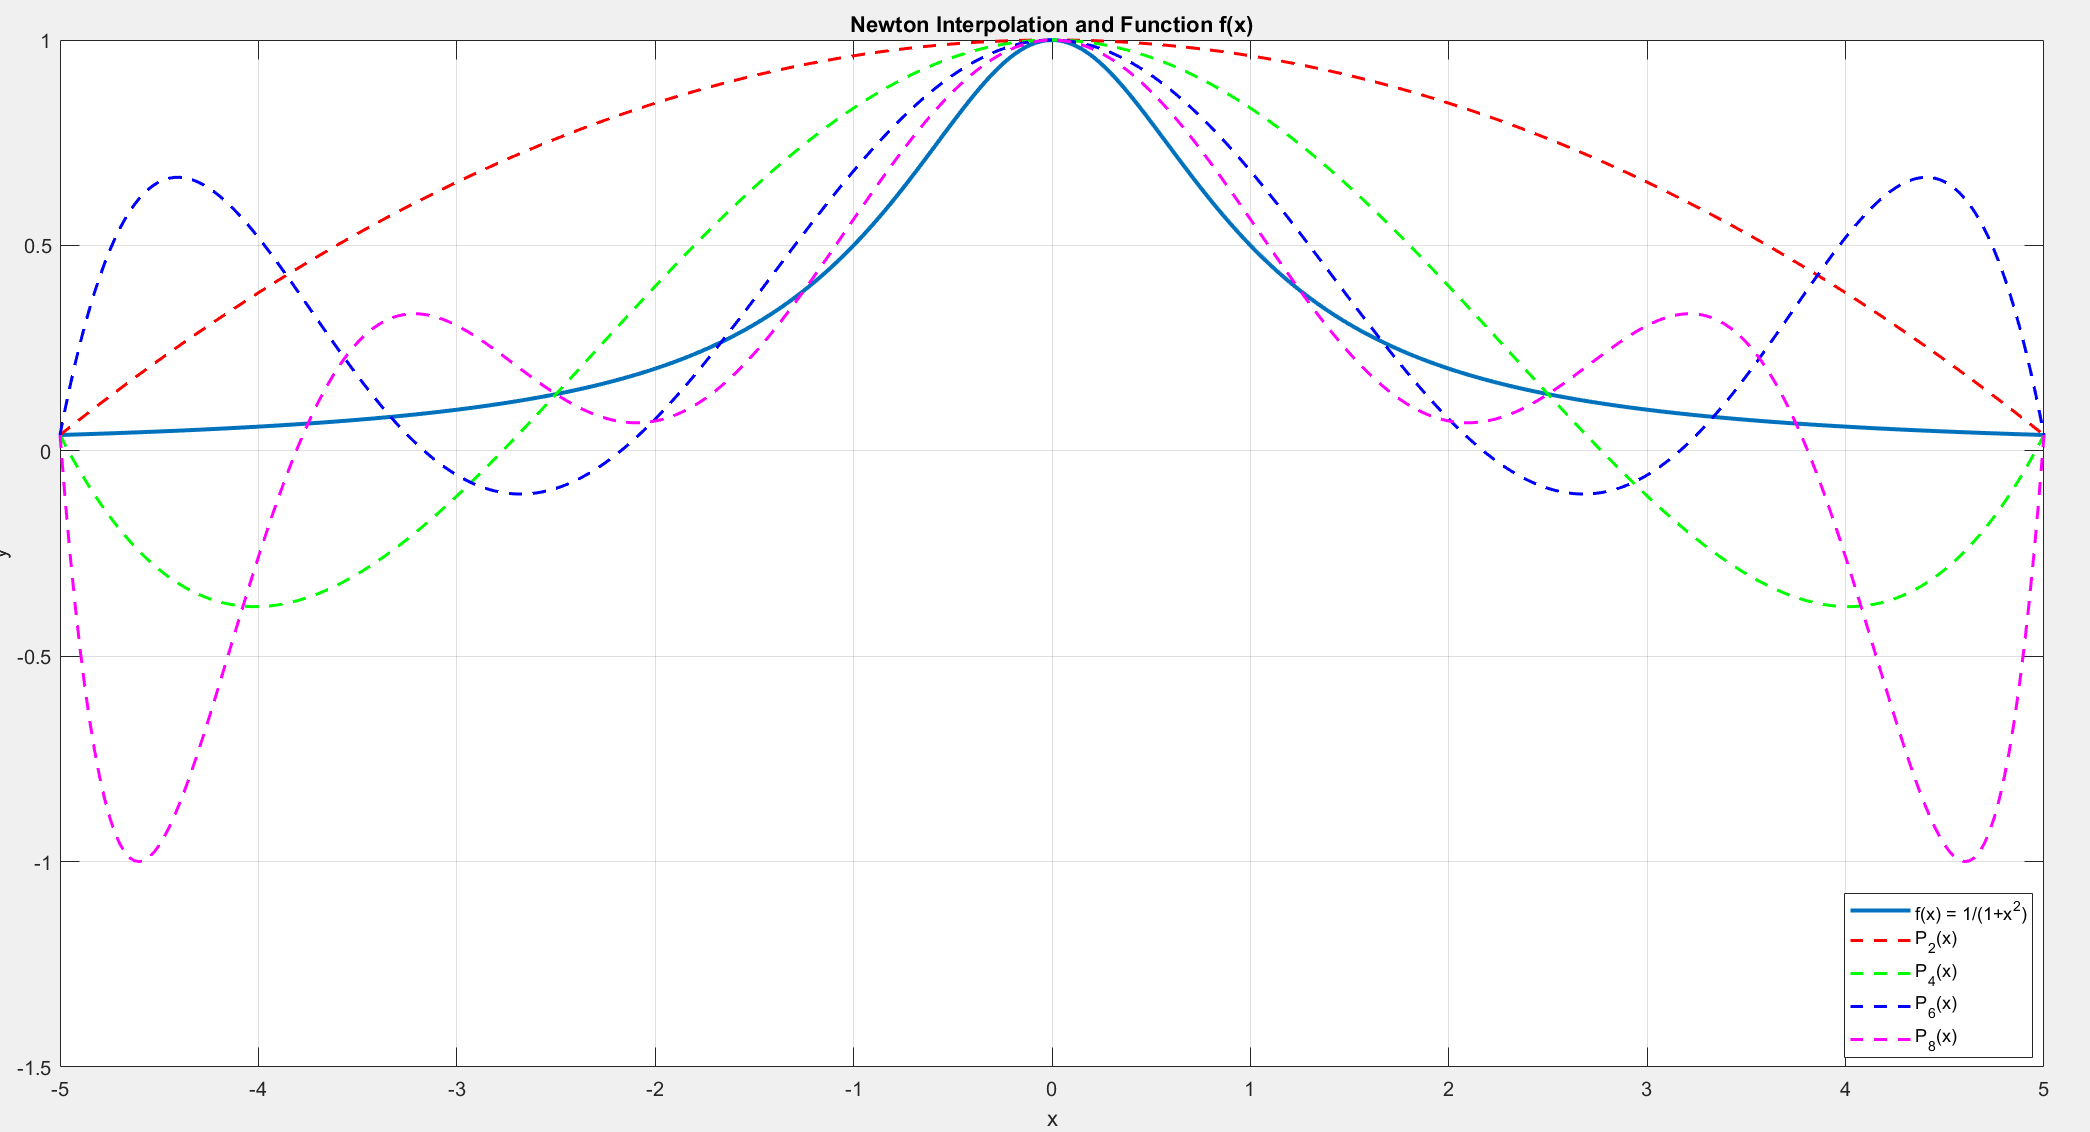
\includegraphics[width=0.7\textwidth]{runge1.png}
    \caption{Newton interpolation and Runge function for different $n$ values.}
    \label{fig:runge_plot}
\end{figure}

The polynomials, $P_2(x), P_4(x), P_6(x), P_8(x)$, show increasing oscillations, especially near $x = -5$ and $x = 5$, confirming that increasing the number of interpolation points does not necessarily improve the accuracy across the entire domain.

\subsection{Conclusion}

In conclusion, the experiment successfully reproduces the Runge phenomenon through the implementation of Newton interpolation. The results demonstrate the limitations of polynomial interpolation using evenly spaced points, particularly for higher-degree polynomials. While the interpolation performs well near the center of the interval, it diverges near the boundaries, causing large oscillations as $n$ increases. This underscores the importance of considering alternative interpolation strategies, such as Chebyshev nodes, for mitigating these issues in practical applications.





\section{Problem C}
This report analyzes the implementation and results of Chebyshev interpolation applied to the Runge function. The Runge function, defined as $f(x) = \frac{1}{1 + 25x^2}$ on the interval $[-1,1]$, is a classical example used to demonstrate Runge's phenomenon in polynomial interpolation.
\subsection{Methodology}
The implementation utilizes Newton interpolation at Chebyshev nodes. The key components include:
\begin{itemize}
\item The Runge function: $f(x) = \frac{1}{1 + 25x^2}$.
\item Chebyshev nodes generation for $n = 5, 10, 15,$ and $20$.
\item Newton interpolation method applied at these nodes.
\end{itemize}
The Chebyshev nodes are calculated using the formula:
\[x_k = \cos\left(\frac{(2k+1)\pi}{2n}\right), \quad k = 0,1,\ldots,n-1\]
\subsection{Results and Analysis}
\begin{figure}[H]
    \centering
    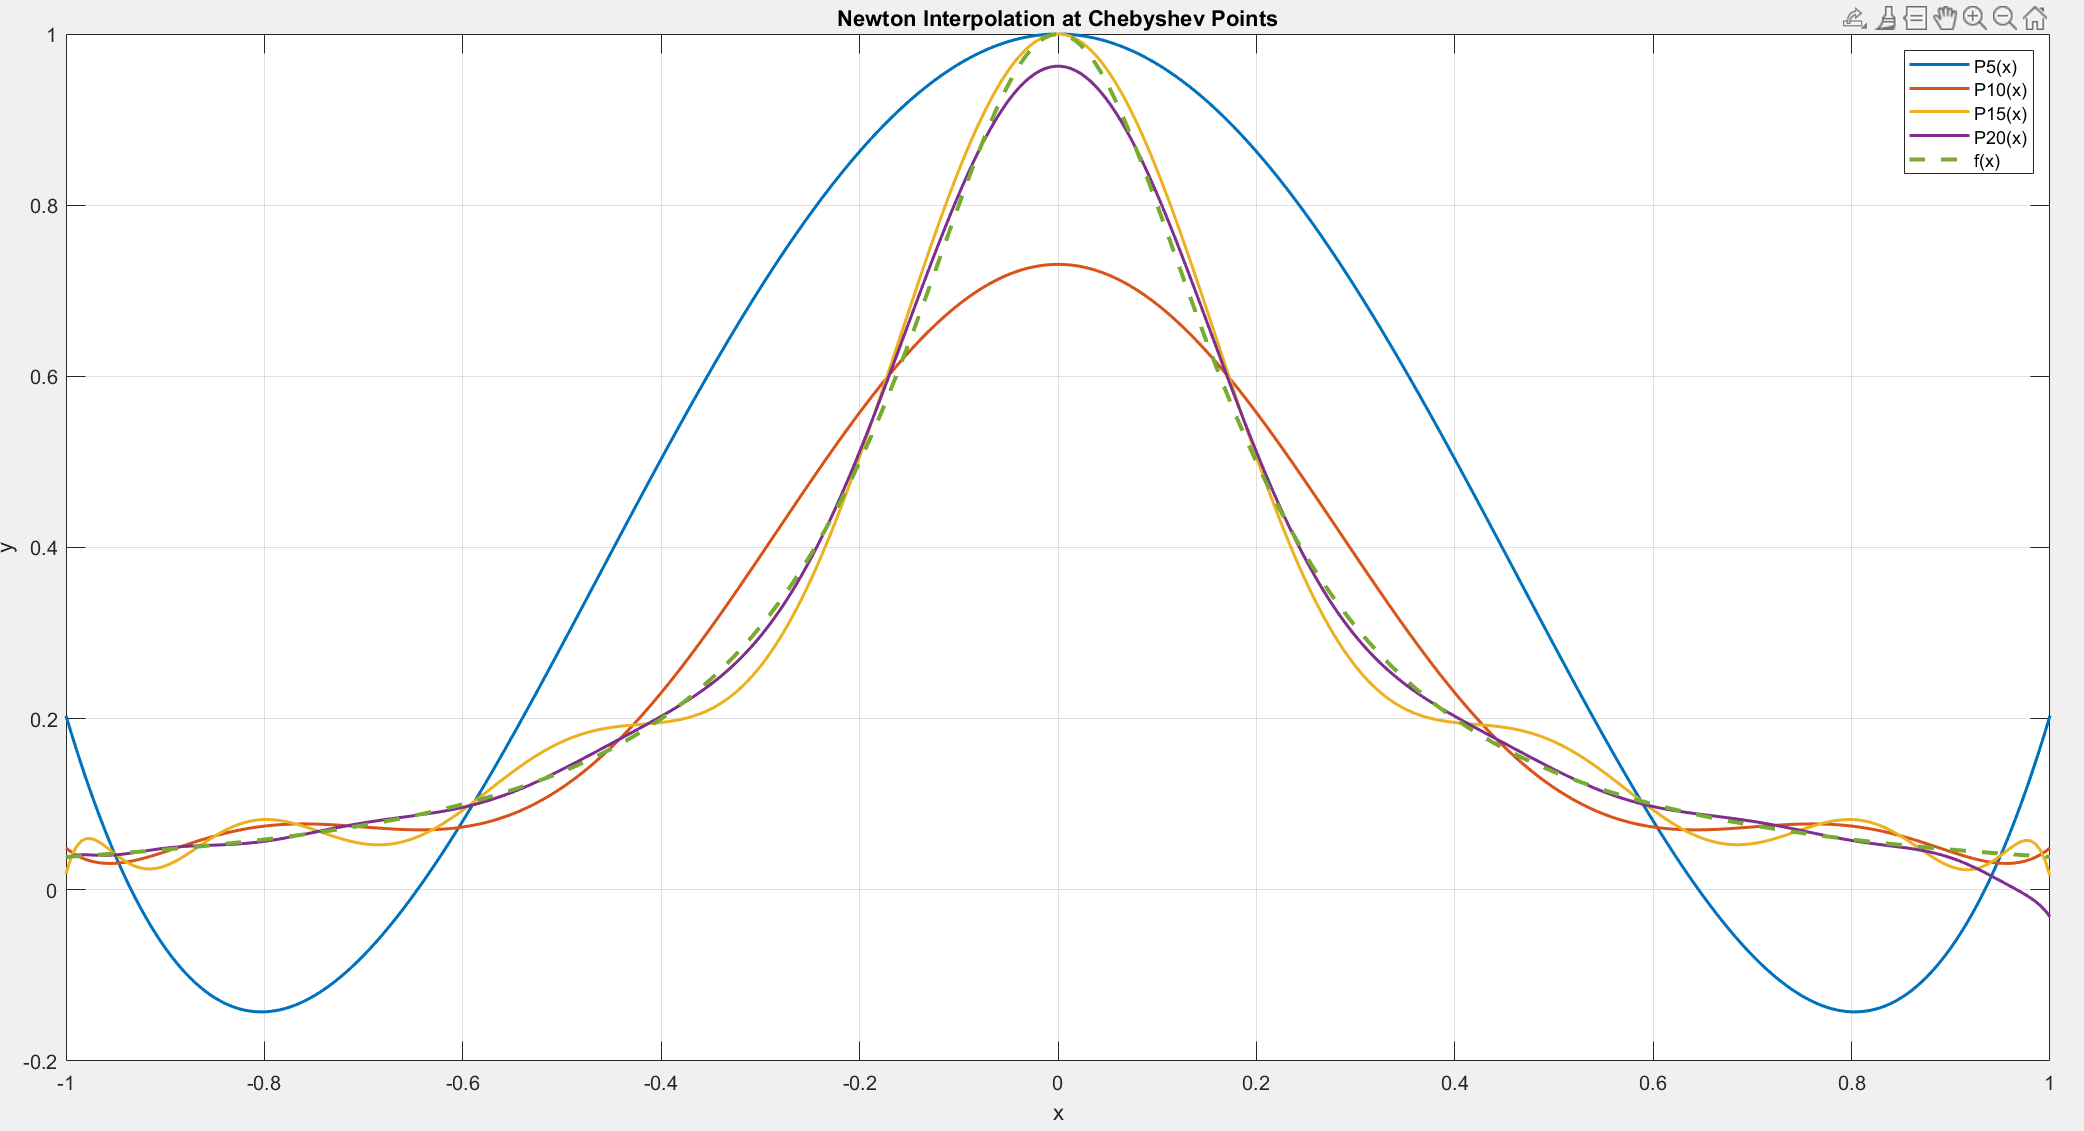
\includegraphics[width=0.7\textwidth]{runge2.png}
    \caption{Chebyshev interpolation and Runge function for different $n$ values.}
    \label{fig:runge_plot}
\end{figure}
The graphical results in Figure 2 demonstrate several key observations:
\begin{enumerate}
\item \textbf{Convergence}: As $n$ increases from 5 to 20, the interpolating polynomials ($P_5(x)$, $P_{10}(x)$, $P_{15}(x)$, and $P_{20}(x)$) show progressively better approximation to the original function.

\item \textbf{Accuracy}: The interpolation becomes particularly accurate for $n=15$ and $n=20$, with minimal deviation from the original function (shown as the dashed green line).
\end{enumerate}

\subsection{Conclusion}
The implementation successfully demonstrates the superiority of Chebyshev interpolation over standard polynomial interpolation for the Runge function. The use of Chebyshev nodes effectively mitigates Runge's phenomenon, providing stable and accurate approximations even at higher degrees.
Key findings include:
\begin{itemize}
\item Increased stability compared to equidistant interpolation.
\item Progressive improvement with increasing polynomial degree.
\item Effective control of endpoint oscillations.

\end{itemize}





\section{Problem D}
Given the following time, displacement, and velocity data points, we are tasked with using Hermite interpolation to model the car's motion:

\begin{table}[H]
    \centering
    \begin{tabular}{|c|c|c|}
        \hline
        Time (s) & Displacement (ft) & Velocity (ft/s) \\ \hline
        0        & 0                 & 75              \\
        3        & 225               & 77              \\
        5        & 383               & 80              \\
        8        & 623               & 74              \\
        13       & 993               & 72              \\ \hline
    \end{tabular}
    \caption{Time, displacement, and velocity data}
\end{table}

The velocity values provided represent the first derivative of the displacement with respect to time.

\subsection{Methodology}

We use Hermite interpolation, which is particularly useful for cases where we have both the function values (displacement) and the derivative values (velocity) at the interpolation points. The Hermite polynomial is constructed based on these data points to predict the displacement and velocity at any given time within the range of the data.

The C++ program provided uses the following key steps:

\begin{enumerate}
    \item Construct the Hermite polynomial using the provided time, displacement, and velocity data.
    \item Interpolate the displacement at \( t = 10 \) seconds using the Hermite polynomial.
    \item Compute the velocity (first derivative of the Hermite polynomial) at \( t = 10 \) seconds.
    \item Check whether the car's velocity exceeds 81 ft/s (55 miles per hour) at any point between \( t = 0 \) and \( t = 13 \) seconds.
\end{enumerate}

\subsection{Results}

\subsubsection{Part (a): Predicted Position and Velocity at \( t = 10 \)}

The predicted displacement and velocity at \( t = 10 \) seconds are as follows:

\begin{itemize}
    \item \textbf{Predicted position:} 742.502839 feet
    \item \textbf{Predicted velocity:} 48.000000 feet/second
\end{itemize}

The position of the car at \( t = 10 \) seconds is approximately 742.50 feet, and its velocity is 48.00 ft/s, which is below the speed limit of 81 ft/s.

\subsubsection{Part (b): Speed Limit Exceedance}

The program further checks if the car exceeds a speed of 81 ft/s at any point between \( t = 0 \) and \( t = 13 \) seconds. The result is as follows:

\begin{itemize}
    \item The car exceeds the speed limit of 81 ft/s at \( t = 11.40 \) seconds.
\end{itemize}

Thus, the car reaches a speed greater than 55 miles per hour at approximately \( t = 11.40 \) seconds.

\subsection{Conclusion}

Using Hermite interpolation, we successfully predicted the car's position and velocity at \( t = 10 \) seconds and determined that the car exceeds the speed limit of 55 miles per hour at \( t = 11.40 \) seconds. Hermite interpolation proves to be an effective method for modeling motion when both displacement and velocity data are available.




\section{Problem E}
We analyze the growth of two samples of larvae, Sp1 and Sp2, reared on young and mature oak leaves, respectively. The data provides the average weight of the larvae at various times within the first 28 days after birth. We use Newton's interpolation formula to approximate the average weight curve for each sample and predict their weights after an additional 15 days.

\subsection{Data}
The data for the average weight of the larvae at different days is as follows:

\begin{table}[h]
\centering
\begin{tabular}{|c|c|c|}
\hline
Day & Sp1 & Sp2 \\
\hline
0 & 6.67 & 6.67 \\
6 & 17.3 & 16.1 \\
10 & 42.7 & 18.9 \\
13 & 37.3 & 15.0 \\
17 & 30.1 & 10.6 \\
20 & 29.3 & 9.44 \\
28 & 28.7 & 8.89 \\
\hline
\end{tabular}
\caption{Average weight of larvae at different days.}
\end{table}

\subsection{Methodology}
We use Newton's interpolation formula to approximate the average weight curve for each sample. Newton's interpolation polynomial is given by:
\[ P(x) = f(x_0) + f[x_0, x_1](x - x_0) + f[x_0, x_1, x_2](x - x_0)(x - x_1) + \cdots \]
where \( f[x_i, x_{i+1}, \ldots, x_n] \) are the divided differences.

\subsection{Results}
The Newton's interpolating polynomial curves for Sp1 and Sp2 are as follows:

\begin{figure}[H]
    \centering
    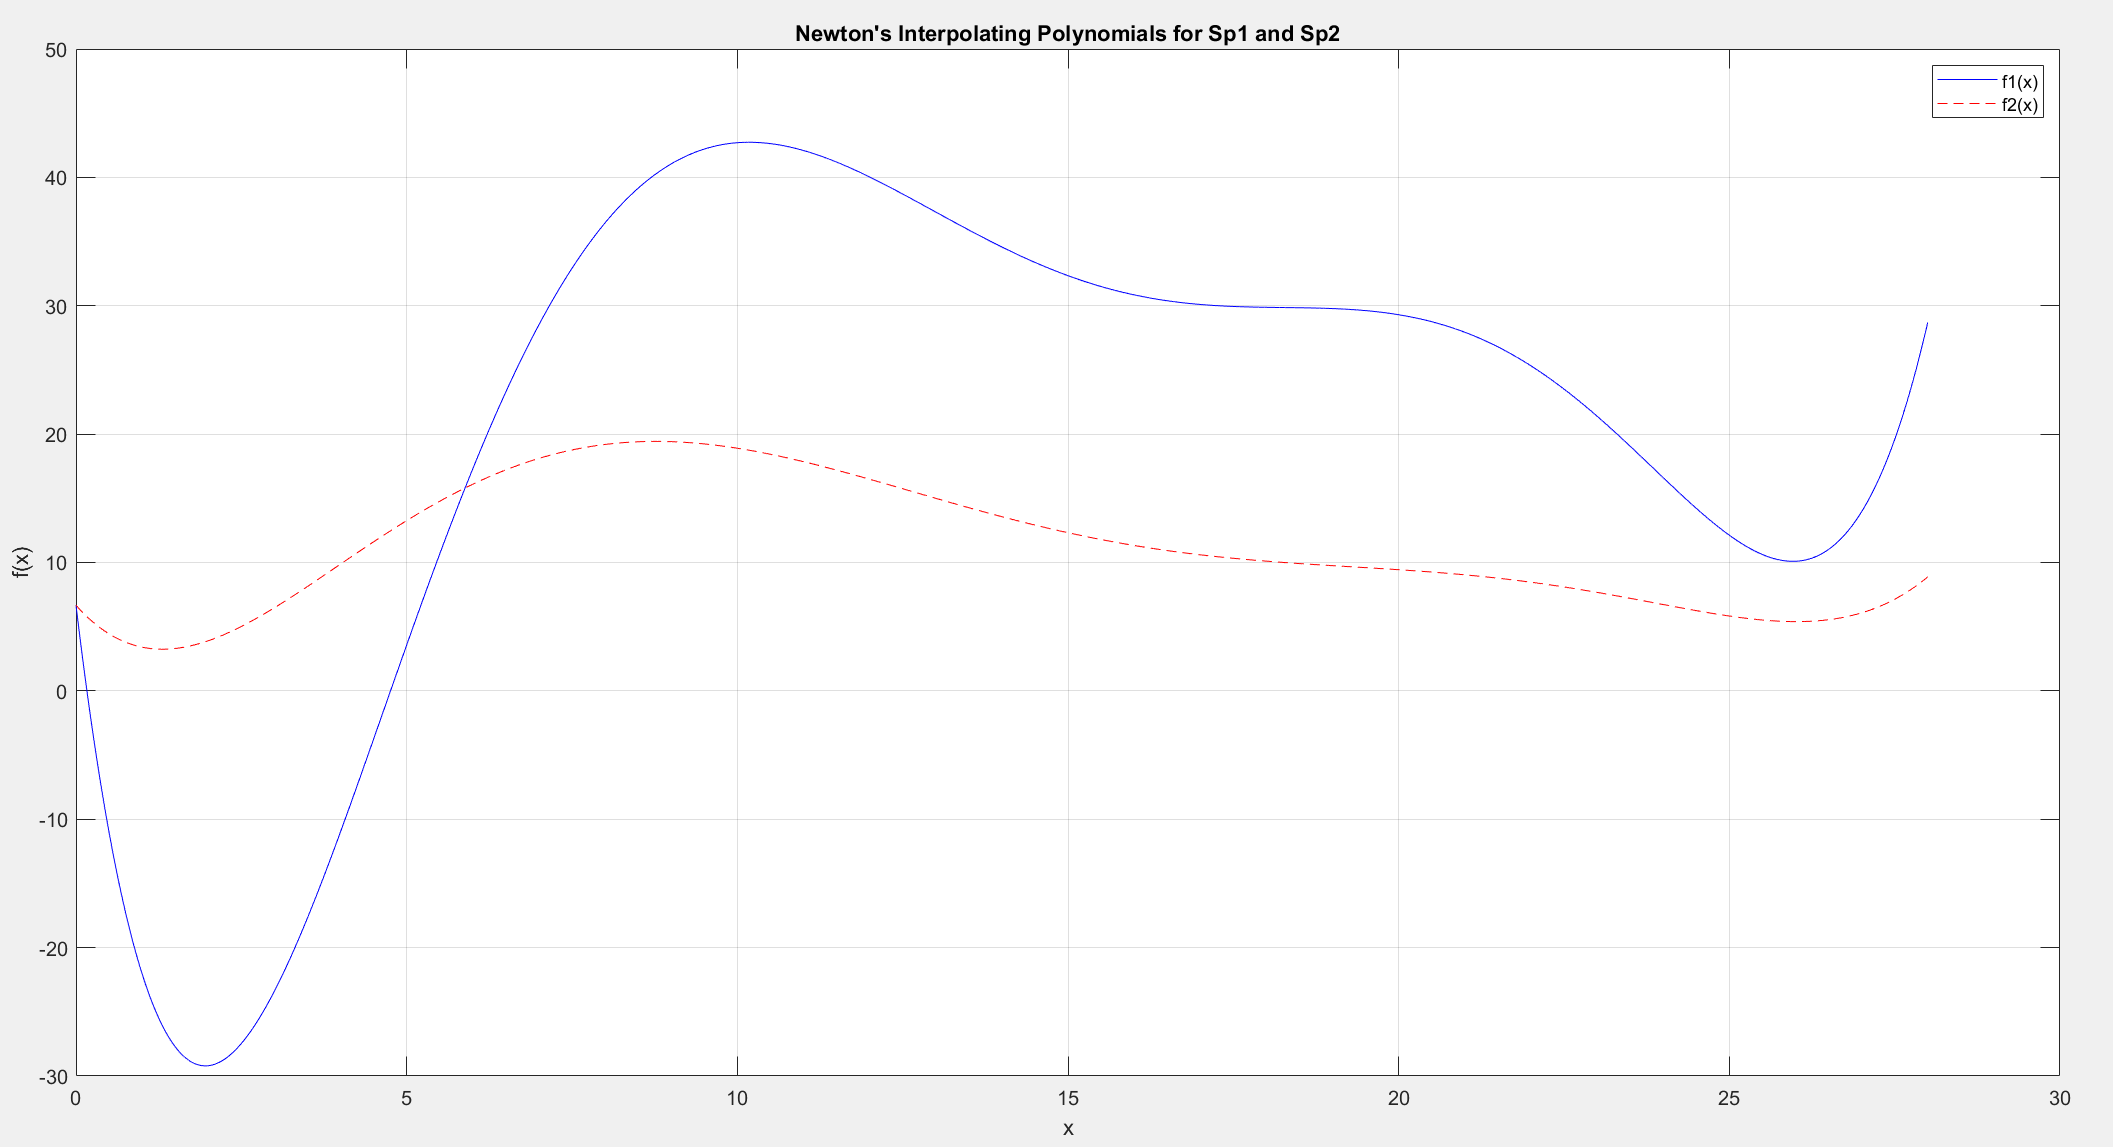
\includegraphics[width=0.8\textwidth]{sp.png}
    \caption{Heart approximation with \(m = 10\)}
    \label{fig:heart10}
\end{figure}

\subsubsection{Predictions}
Using these polynomials, we predict the weights of Sp1 and Sp2 at day 43.
\[ \text{Prediction for Sp1 weight at day 43: } 14640.3 \]
\[ \text{Prediction for Sp2 weight at day 43: } 2981.48 \]

\subsection{Discussion}
The predictions indicate that both samples of larvae will experience a significant increase in weight after another 15 days. However, such high weights are not biologically plausible for the larvae, suggesting that the interpolation polynomials may not accurately model the weight gain beyond the given data range. It is likely that the larvae will not survive past day 28, as their weight would not continue to increase indefinitely.

\subsection{Conclusion}
The use of Newton's interpolation formula provides a mathematical model for the growth of the larvae samples. While the predictions for day 43 are mathematically derived, they may not reflect the actual biological growth patterns of the larvae. It is important to consider the limitations of polynomial interpolation when applying it to real-world data, especially outside the range of the given data points.



\section{Problem F}
This is a C++ program designed to approximate the shape of a heart using cubic Bezier curves. The program generates marker points on the heart curve, calculates tangents at these points, fits cubic Bezier curves, and plots the resulting curves using Gnuplot.

\subsection{Code Analysis}

\subsubsection{Marker Point Generation}
The function \texttt{generateMarkers} generates marker points on the heart curve. It takes an integer \texttt{m} as input, which determines the number of segments into which the curve is divided. The heart curve is defined parametrically by the equations:
\[ x = 16 \sin^3(t) \]
\[ y = 13 \cos(t) - 5 \cos(2t) - 2 \cos(3t) - \cos(4t) \]
where \(t\) ranges from \(0\) to \(2\pi\). The function iterates over this range, dividing it into \(m\) equal parts, and calculates the corresponding \(x\) and \(y\) coordinates for each point.

\subsubsection{Tangent Calculation}
The \texttt{calculateTangents} function computes the tangents at the marker points. It takes a vector of points as input and returns a vector of tangent vectors. For each marker point, except the first and last, the tangent is calculated as the average of the vectors from the current point to the next and from the previous point to the current. For the first and last points, the tangents are simply the vectors to the next and previous points, respectively.

\subsubsection{Bezier Curve Fitting}
The \texttt{fitCurve} function, which is part of the \texttt{BezierInterpolation} class, fits cubic Bezier curves to the marker points and their tangents. This function is not explicitly defined in the provided code, but it is assumed to use the De Casteljau's algorithm or a similar method to determine the control points of the Bezier curves that best fit the marker points and their tangents.

\subsubsection{Gnuplot Script Generation}
The \texttt{generateGnuplotScript} function creates a Gnuplot script that plots the Bezier curves. It takes the \texttt{BezierInterpolation} object, the vector of Bezier curves, and a filename as input. The function sets up the Gnuplot terminal and output file, then plots each Bezier curve by evaluating the curve at increments of \(0.01\) from \(t = 0\) to \(t = 1\).

\subsection{Results and Discussion}
The program generates three Gnuplot scripts for different values of \(m\) (10, 40, and 160), which correspond to the number of segments used to approximate the heart curve. The resulting plots show how the approximation of the heart shape improves as \(m\) increases, with more segments leading to a smoother curve that more closely resembles the heart shape.

\begin{figure}[H]
    \centering
    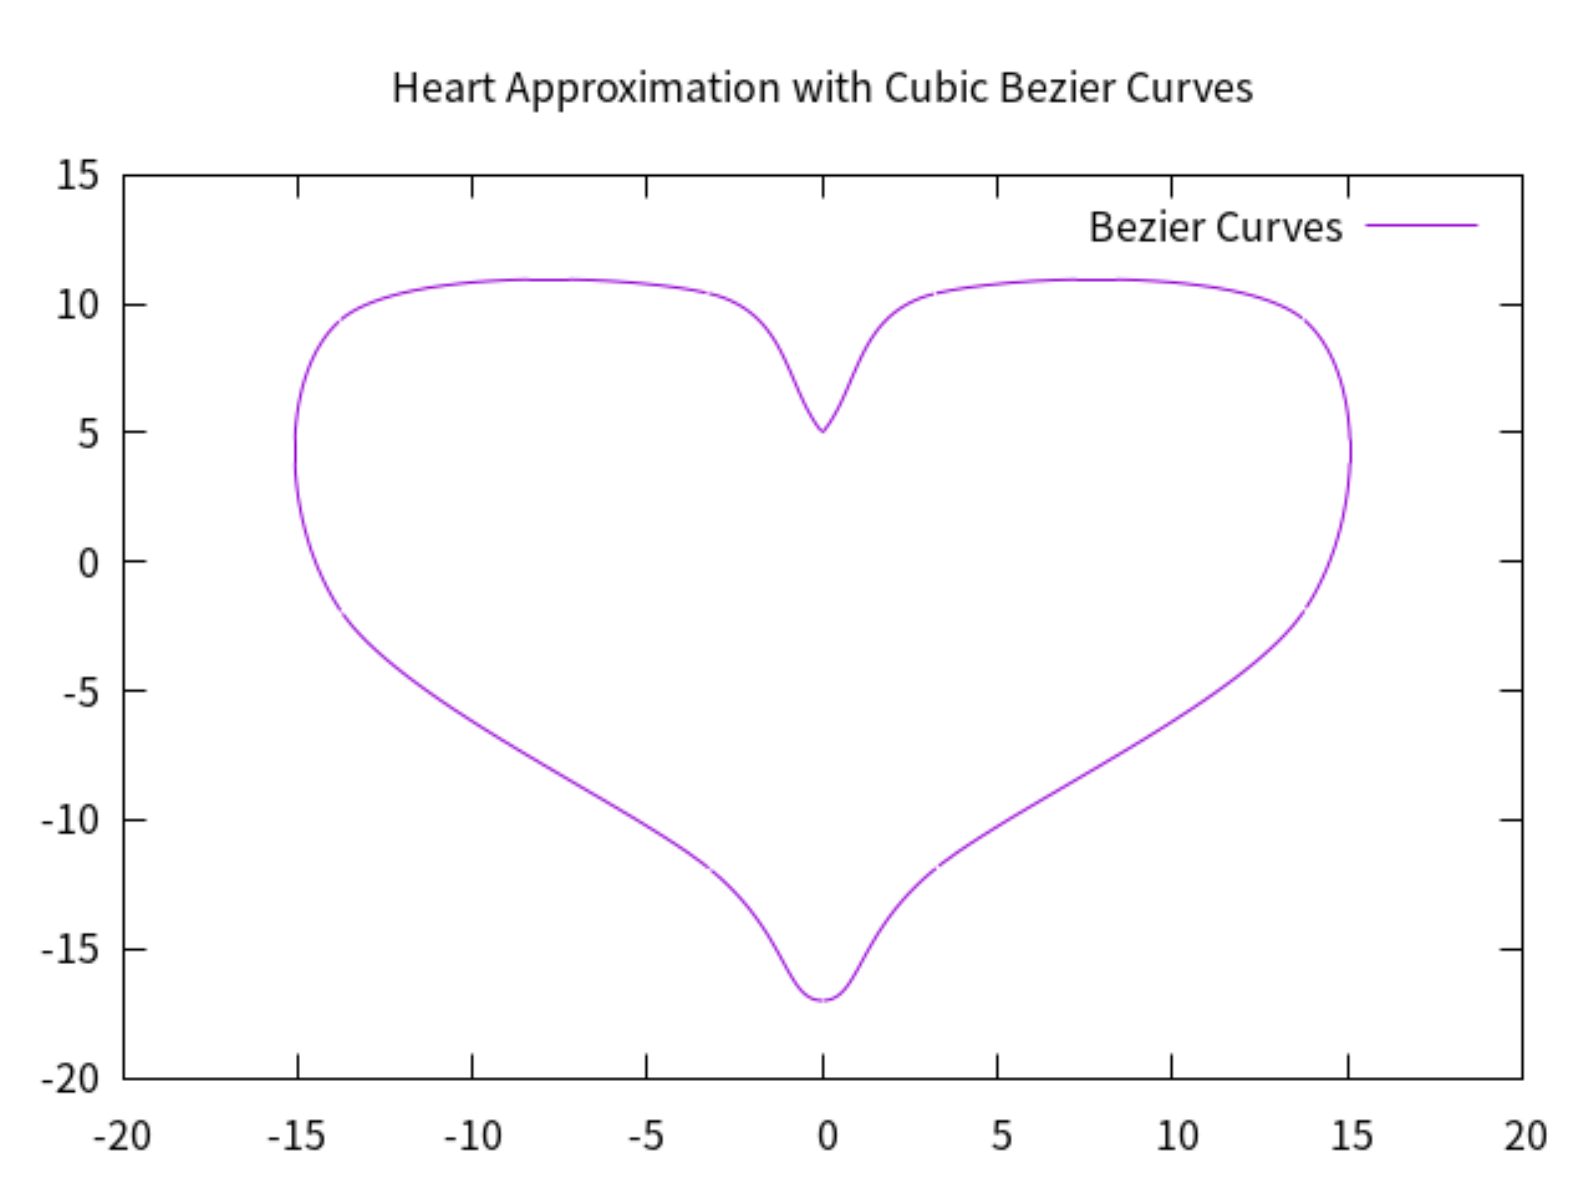
\includegraphics[width=0.7\textwidth]{10.png}
    \caption{Heart approximation with \(m = 10\)}
    \label{fig:heart10}
\end{figure}

\begin{figure}[H]
    \centering
    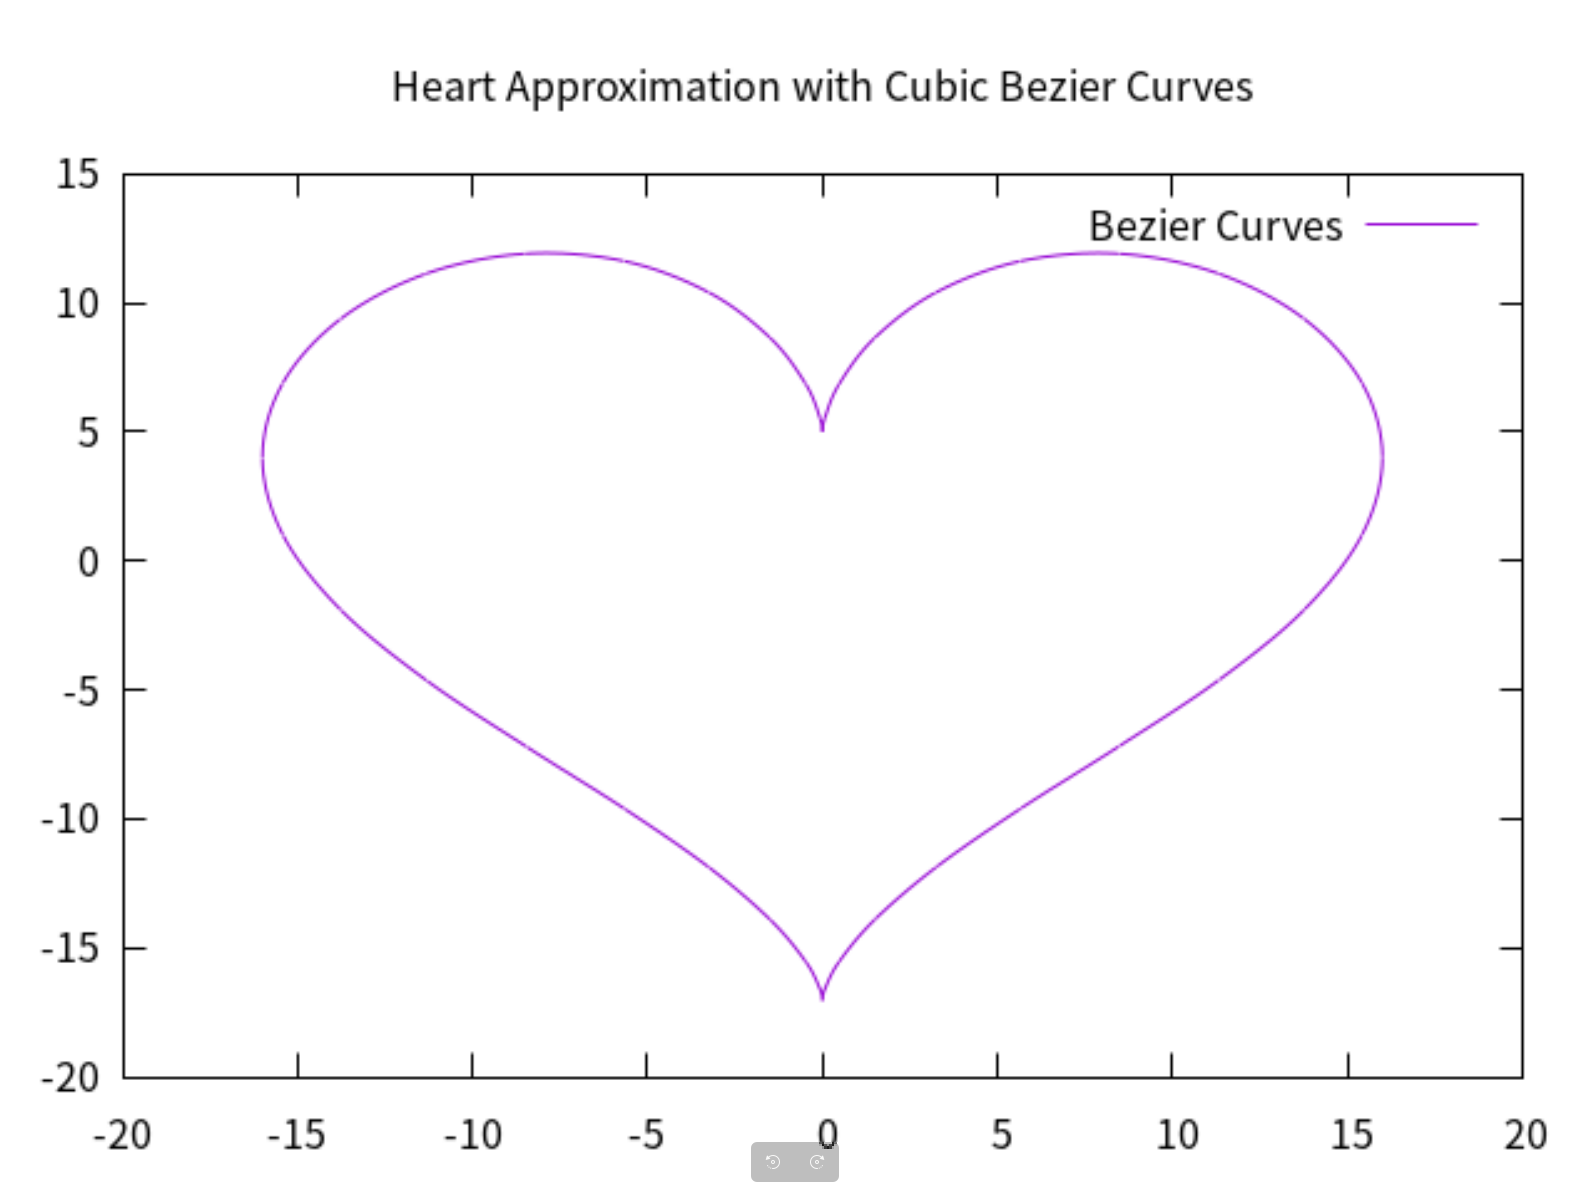
\includegraphics[width=0.7\textwidth]{40.png}
    \caption{Heart approximation with \(m = 40\)}
    \label{fig:heart40}
\end{figure}

\begin{figure}[H]
    \centering
    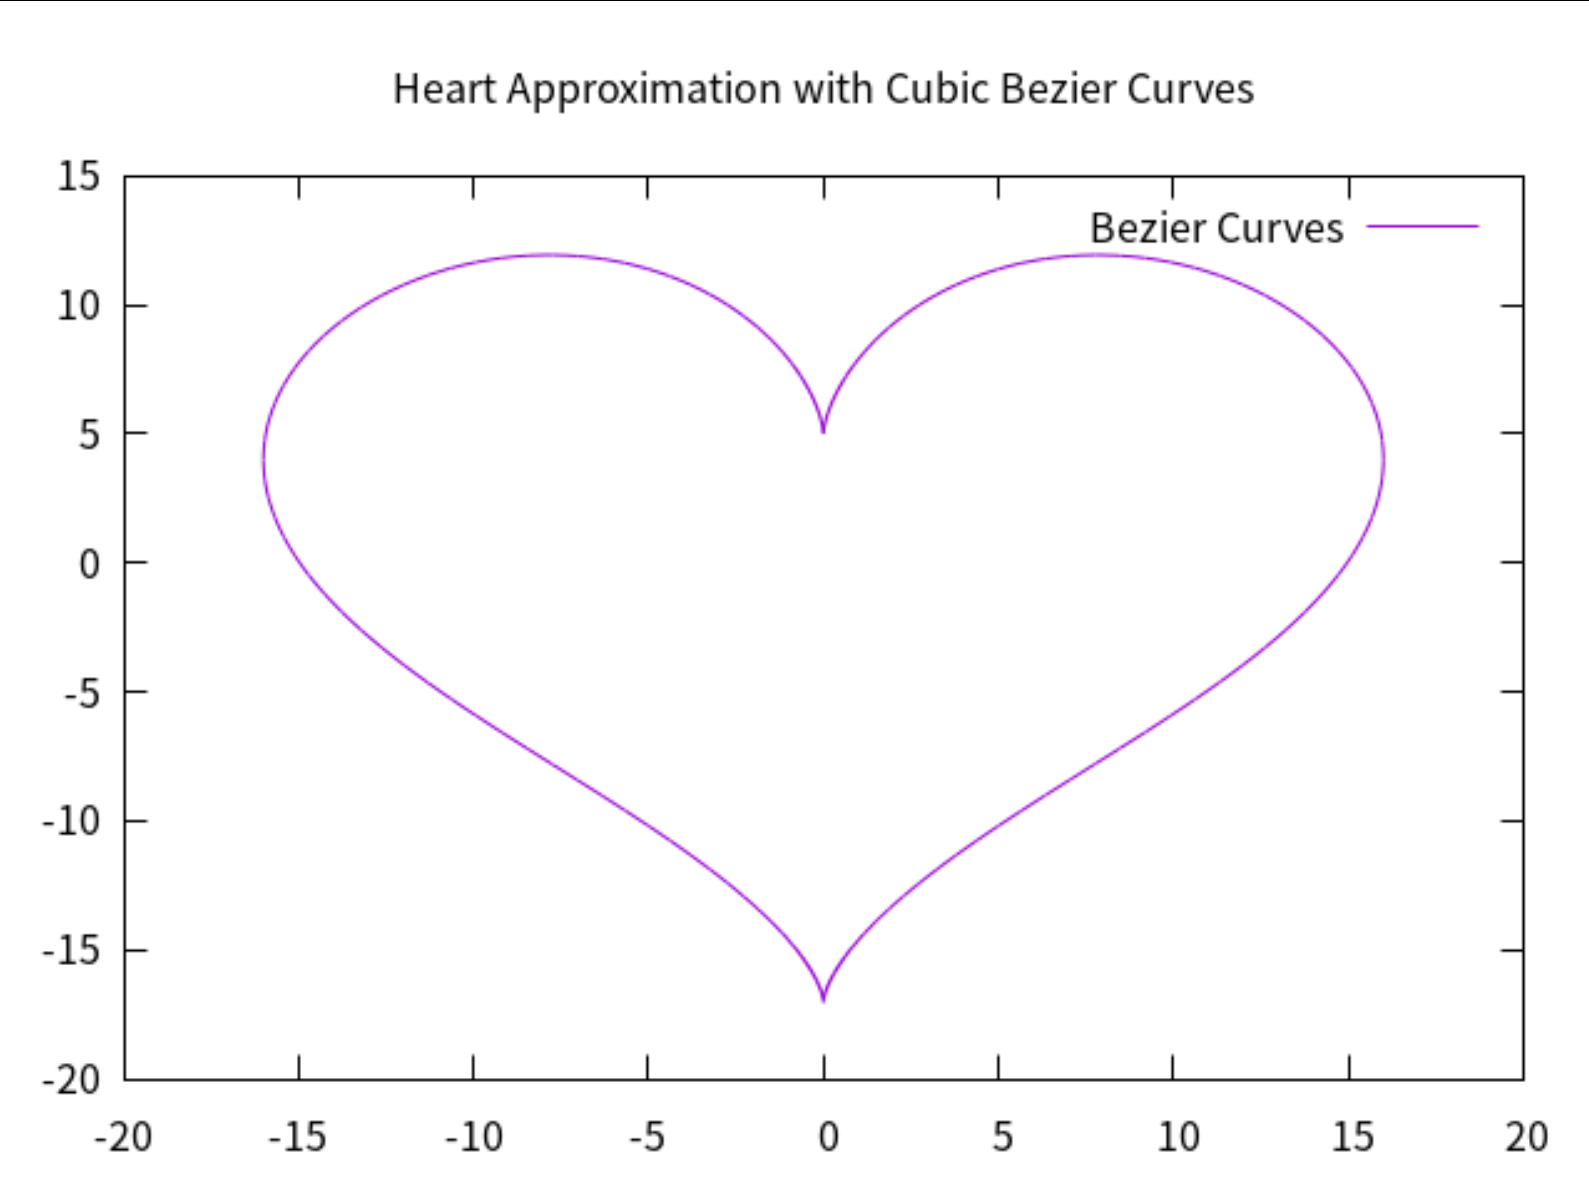
\includegraphics[width=0.7\textwidth]{160.png}
    \caption{Heart approximation with \(m = 160\)}
    \label{fig:heart160}
\end{figure}

\subsection{Conclusion}
The provided C++ program is a robust method for approximating complex curves, such as the heart shape, using cubic Bezier curves. By varying the number of segments, the program demonstrates the flexibility of Bezier curves in capturing the nuances of a curve. The use of Gnuplot for plotting allows for visualization of the approximation, making it a valuable tool in computer graphics and related fields.


\end{document}
